
%\section{Experimental Details and Additional Results}

\section{Experimental Details and Additional Results}
\label{sec:exper-deta-addit}


\begin{figure}[htp]
		\centering
		 	\subfigure[Two cosine functions.]{
			\centering
			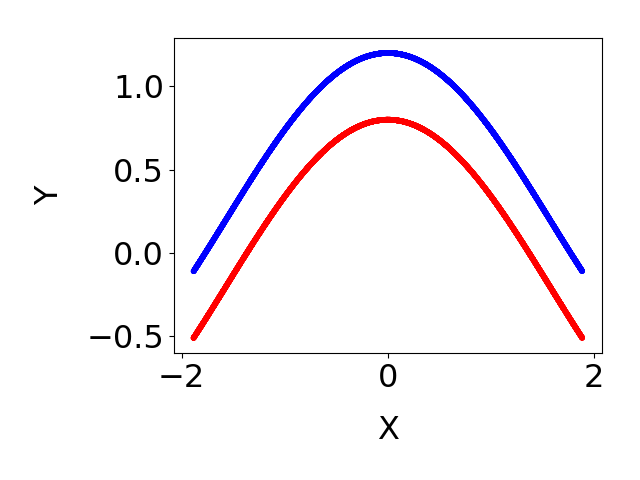
\includegraphics[scale=0.34]{Figures/two_cosine.png}
			\label{fig:two-cosine}}
            \hspace{0.01in}
        	\subfigure[The local elasticity of two-layer neural nets fitting these two cosine functions.]{
			\centering
			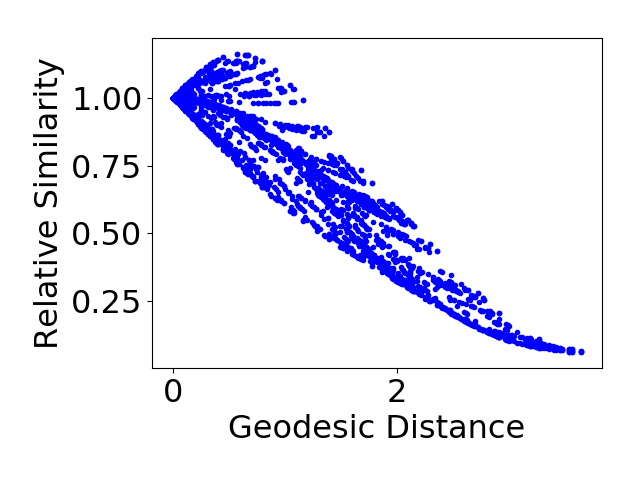
\includegraphics[scale=0.34]{Figures/two_cosine_MLPNet_ripple_random.png}
			\label{fig:two-cosine-NNs}}
			\hspace{0.01in}
			\subfigure[The double helix function.]{
			\centering
			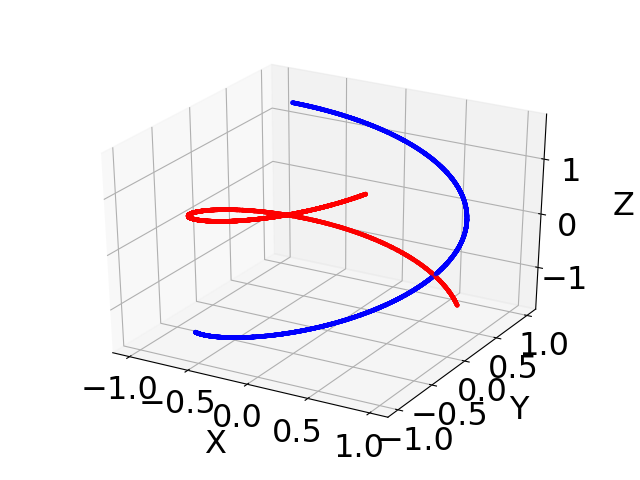
\includegraphics[scale=0.34]{Figures/double_helix.png}
			\label{fig:double-helix}}
            \hspace{0.01in}
        	\subfigure[The local elasticity of two-layer neural nets fitting the double helix function.]{
			\centering
			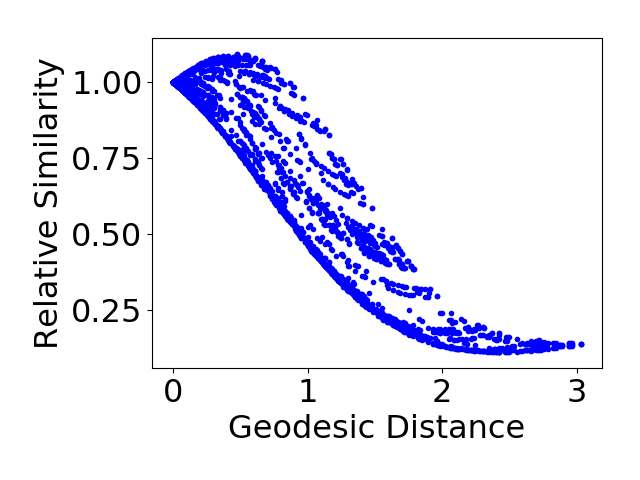
\includegraphics[scale=0.34]{Figures/double_helix_MLPNet_ripple_random.png}
			\label{fig:double-helix-NNs}}
			\hspace{0.01in}
			\subfigure[Two cycle functions.]{
			\centering
			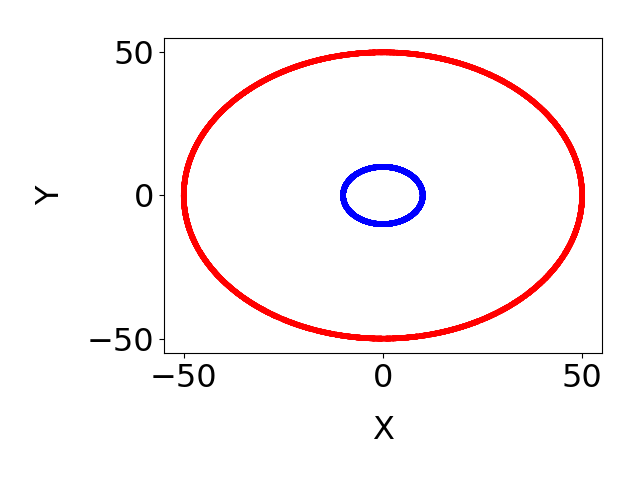
\includegraphics[scale=0.34]{Figures/two_cycles.png}
			\label{fig:two-cycles}}
            \hspace{0.01in}
        	\subfigure[The local elasticity of two-layer neural nets fitting two cycle functions.]{
			\centering
			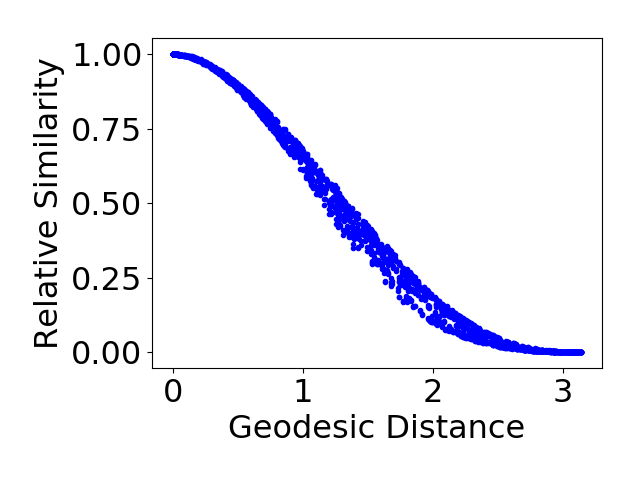
\includegraphics[scale=0.34]{Figures/two_cycles_MLPNet_ripple_random.png}
			\label{fig:two-cyles-NNs}}
			\hspace{0.01in}
			\subfigure[Two sphere functions.]{
			\centering
			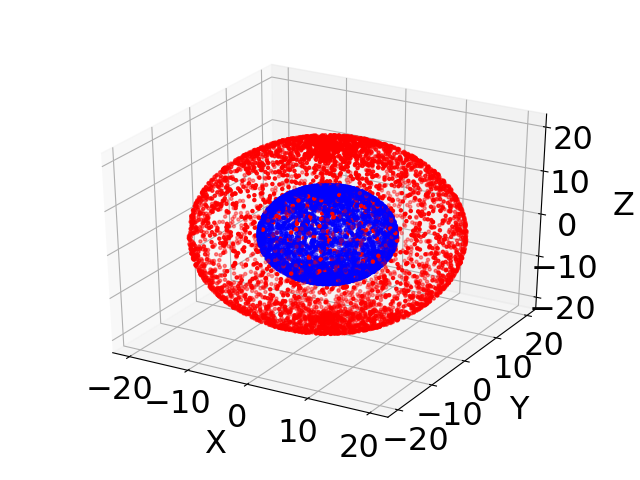
\includegraphics[scale=0.34]{Figures/two_sphere.png}
			\label{fig:two-sphere}}
            \hspace{0.01in}
        	\subfigure[The local elasticity of two-layer neural nets fitting two sphere functions.]{
			\centering
			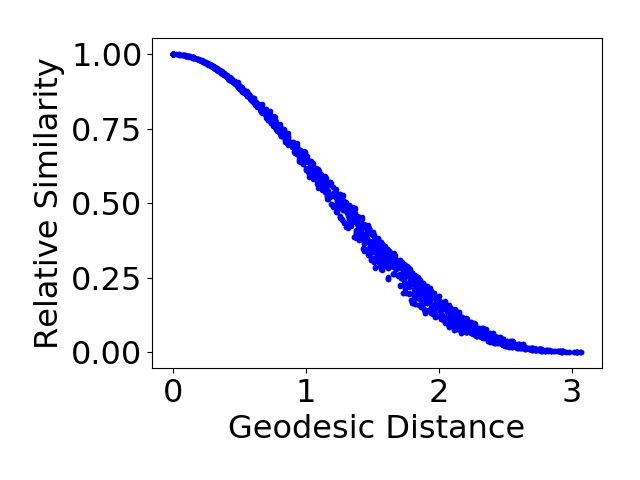
\includegraphics[scale=0.34]{Figures/two_sphere_MLPNet_ripple_random.png}
			\label{fig:two-sphere-NNs}}
			\hspace{0.01in}
		\caption{More simulations of the local elasticity.} 
		\label{fig:more-simulations}
\end{figure}

\begin{figure}[!htp]
		\centering
		\subfigure[A tabby cat.]{
			\centering
			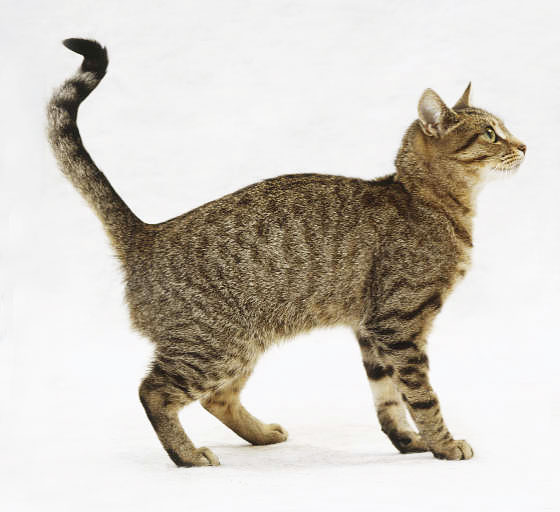
\includegraphics[scale=0.19]{Figures/tabby_cat_n02123045_10001.JPEG}
			\label{fig:tabby-cat}}
        \hspace{0.01in}
        \subfigure[A tiger cat.]{
			\centering
			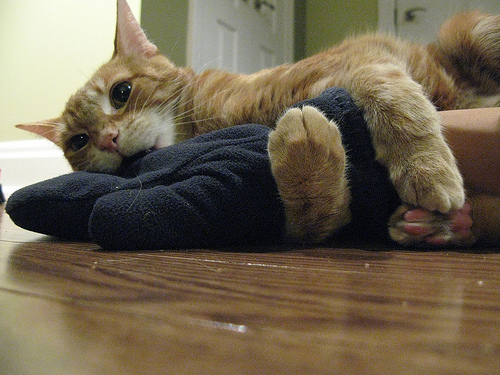
\includegraphics[scale=0.25]{Figures/tiger_cat_n02123159_1011.JPEG}
			\label{fig:tiger-cat}}
        \hspace{0.01in}
         \subfigure[A warplane.]{
			\centering
			
\includegraphics[scale=0.18]{Figures/plane_n04552348_10078.JPEG}
			\label{fig:warplane}}
        \caption{Simulations in real data. We show specific examples for a tabby cat, a tiger cat and a warplane.}
		\label{fig:real-simulations}
\end{figure}

\begin{figure}[t]
		\centering
		\subfigure[A tabby cat (train).]{
			\centering
			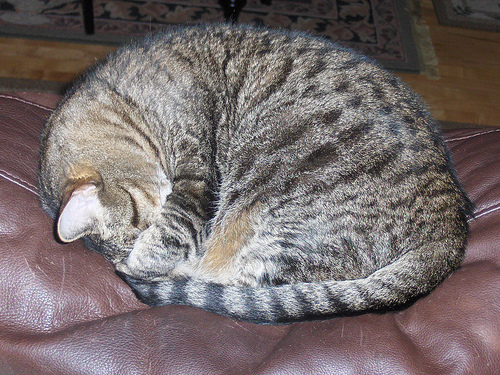
\includegraphics[scale=0.27]{Figures/tabby_cat_1.JPEG}
			\label{fig:tabby-cat-1}}
        \hspace{0.01in}
         \subfigure[A warplane (train).]{
			\centering
			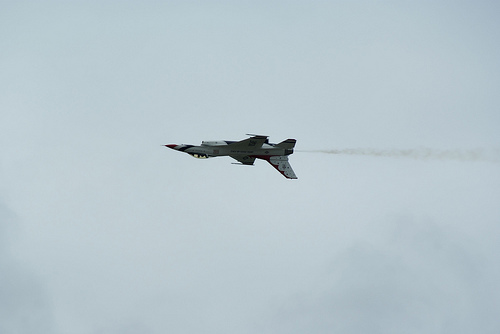
\includegraphics[scale=0.3]{Local-Elasticity/Figures/warplane_1.JPEG}
			\label{fig:warplane-1}}
		\subfigure[A tabby cat (test).]{
			\centering
			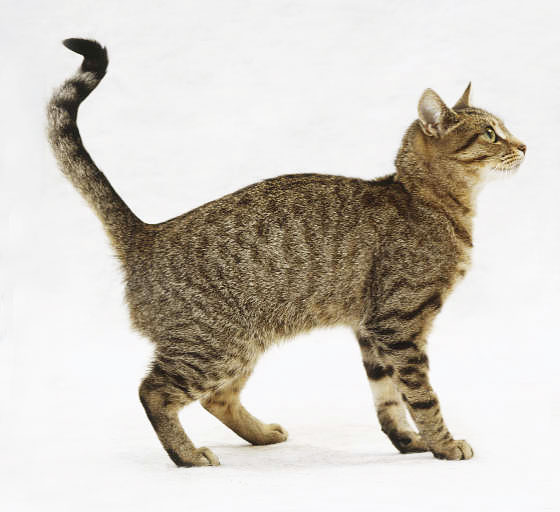
\includegraphics[scale=0.18]{Figures/tabby_cat_0.JPEG}
			\label{fig:tabby-cat-0}}
        \hspace{0.01in}
         \subfigure[A warplane (test).]{
			\centering
			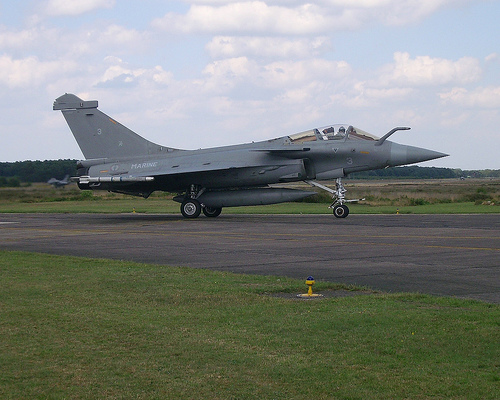
\includegraphics[scale=0.23]{Local-Elasticity/Figures/warplane_0.JPEG}
			\label{fig:warplane-0}}
		\subfigure[A tree frog (test).]{
			\centering
			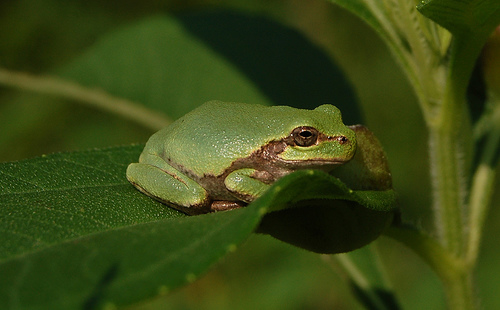
\includegraphics[scale=0.3]{Figures/tree_frog_0.JPEG}
			\label{fig:tree-frog-0}}
        \hspace{0.01in}
        \caption{Simulations showing local elasticity with mini-batch SGD.}
		\label{fig:real-simulations}
\end{figure}

\subsection{Construction of the Synthetic Examples in Figure~\ref{fig:simulations}}
\label{subsec:functions}
The blue examples in the torus function (Figure \ref{fig:torus}) can be defined parametrically by:
\begin{equation}
\begin{aligned}
 x(\theta) &= (8 + \sin(4\theta))\cos{\theta} \\
 y(\theta) &= (8 + \sin(4\theta))\sin{\theta} \\
 z(\theta) &= \cos(4\theta)
\end{aligned}
\end{equation}
Similarly, the red examples in the torus function are defined by:
\begin{equation}
\begin{aligned}
 x(\theta) &= (8 - \sin(4\theta))\cos{\theta} \\
 y(\theta) &= (8 - \sin(4\theta))\sin{\theta} \\
 z(\theta) &= -\cos(4\theta)
\end{aligned}
\end{equation}
The blue examples in the two folded boxes function (Figure \ref{fig:two-fold-surface}) are sampled from:
\begin{equation}
\begin{aligned}
 \left| y \right| + 1.2 \left| x \right| = 13\\
 z \in [-1, 1]
\end{aligned}
\end{equation}
Similarly, the red examples in the two folded boxes function are defined as:
\begin{equation}
\begin{aligned}
 \left| y \right| + 1.2 \left| x \right| = 11\\
 z \in [-1, 1]
\end{aligned}
\end{equation}

%\paragraph{Geodesic Distance}
%\label{subsec:geodesic}
Geodesic distance is used to measure the shortest path between two points in a surface, or more generally in a Riemannian manifold. For example, in Figure \ref{fig:simulations}, the geodesic distance for the torus function and the two folded boxes function is the distance in the curve and the distance in the surface rather than the Euclidean distance.

\subsection{More Simulations} 
\label{subsec:more-simulations}
More simulations can be found in Figure \ref{fig:more-simulations}.


%\subsection{\hangfengchange{Simulations in Real Data}}
We further explore the local elasticity of ResNet-152 on ImageNet. We find that, when the pre-trained ResNet-152 are updated on a tabby cat via SGD, the predictions of tiger cats change more drastically than the predictions of warplanes. We randomly pick $50$ examples from the tabby cat synset as updating points, $25$ examples from the tiger cat synset and $25$ examples from the warplane synset as testing points. After updating on a tabby cat, we can get the average change of predictions on the $25$ tiger cats and that on the $25$ warplanes. By conducting a Wilcoxon rank-sum test with SGD updates on $50$ different tabby cats, we find that the average change of the predictions on the tiger cat are significantly more drastic than that on the warplane with a p-value of $0.0007$. The overall average relative similarity between the tiger cats and the tabby cats is $4.4$, while the overall average similarity between the  warplanes and the tabby cats is $6.6$. Note that the relative similarity is computed from the relative KL divergence between the original prediction and the updated prediction. 

Specifically, we find that the change of the predictions (KL divergence of $0.03$) on the tiger cat (Figure \ref{fig:tiger-cat}) is more drastic than that (KL divergence of $0.002$) on the warplane (Figure \ref{fig:warplane}) after a SGD update on the tabby cat (Figure \ref{fig:tabby-cat}), although the Euclidean distance ($511$) between the warplane and the tabby cat is smaller than that ($854$) between the tiger cat and the tabby cat.

Moreover, we conduct a simulation study to examine local elasticity in the case of using mini-batch SGD for updates. Specifically, we consider updating the weights of ResNet-152 in one iteration using two images. The training and test images are displayed in Figure~\ref{fig:real-simulations}. We find that the changes of the predictions on the tabby cat (Figure \ref{fig:tabby-cat-0}, KL divergence of $0.021$) and on the warplane (Figure \ref{fig:warplane-0}, KL divergence of $0.024$) are more substantial than that on the tree frog (Figure \ref{fig:tree-frog-0}, KL divergence of $0.0004$) after an SGD update on the minibatch composed of a tabby cat (Figure \ref{fig:tabby-cat-1}) and a warplane (Figure \ref{fig:warplane-1}).
\subsection{Some Calculations}
%Details of Theoretical Analysis}
\label{sec:deta-theor-analys}



\iffalse

We consider applying SGD to kernel regression:
\[
\sum_{i=1}^N \frac12 (\bw^\top \varphi(\bx_i) - y_i)^2,
\]
which gives
\[
\bw_{t+1} = \bw_t - \eta(\bw^\top \varphi(\bx_i) - y_i) \varphi(\bx_i).
\]
Therefore, the kernel trick gives
\[
\begin{aligned}
f(\bw_{t+1}, \bx_j) &= \bw_{t+1}^\top \varphi(\bx_i)\\
&=\left\langle \bw_t - \eta (\bw_t^\top \varphi(\bx_i) - y_i) \varphi(\bx_i),  \varphi(\bx_j) \right\rangle\\
& = f(\bw_t, \bx_j) - \eta (\bw_t^\top \varphi(\bx_i) - y_i) \left\langle \varphi(\bx_i),  \varphi(\bx_j) \right\rangle\\
& = f(\bw_t, \bx_j) - \eta (\bw_t^\top \varphi(\bx_i) - y_i) K(\bx_i, \bx_j).
\end{aligned}
\]
As such, the change of the prediction on $\bx_j$ is contingent upon $K(\bx_i, \bx_j)$.

\fi


We brief explain how to obtain Equation (\ref{eq:dnn_diff}) under the same assumptions of \citet{li2018learning}.
\[
\begin{aligned}
f(\overline\bx', \bw^+) - f(\bx', \bw) &= \sum_{r=1}^m a_r \sigma((\bw_r^+)^\top \bx') - \sum_{r=1}^m a_r \sigma(\bw_r^\top \bx')\\
&= \sum_{r=1}^m a_r \sigma\left(\left(\bw_r - \eta \frac{\partial \mathcal{L}}{\partial f} a_r \bx \mathbb{I}\{\bw_r^T \bx \ge 0\} \right)^\top \bx' \right) - \sum_{r=1}^m a_r \sigma(\bw_r^\top \bx')\\
&= \sum_{r=1}^m a_r \sigma\left( \bw_r^\top \bx' - \eta \frac{\partial \mathcal{L}}{\partial f} a_r \bx^\top \bx' \mathbb{I}\{\bw_r^T \bx \ge 0\} \right) - \sum_{r=1}^m a_r \sigma(\bw_r^\top \bx')\\
& = \Delta_1 + \Delta_2,
\end{aligned}
\]
where
\[
\begin{aligned}
\Delta_1 &= - \eta \frac{\partial \mathcal{L}}{\partial f} \sum_{r=1}^m \bx^\top \bx' \mathbb{I}\{\bw_r^T \bx \ge 0\} \mathbb{I}\{\bw_r^\top \bx' \ge 0\}\\
&= - \eta \frac{\partial \mathcal{L}}{\partial f}\bx^\top \bx'  \sum_{r=1}^m \mathbb{I}\{\bw_r^T \bx \ge 0\} \mathbb{I}\{\bw_r^\top \bx' \ge 0\}
\end{aligned}
\]
and 
\[
\begin{aligned}
\|\Delta_2\|  &\le \sum_{r=1}^m \left| - a_r \eta \frac{\partial \mathcal{L}}{\partial f} a_r \bx^\top \bx' \mathbb{I}\{\bw_r^T \bx \ge 0\} \right| \cdot \left| \mathbb{I}\left\{ \bw_r^\top \bx' - \eta \frac{\partial \mathcal{L}}{\partial f} a_r \bx^\top \bx' \mathbb{I}\{\bw_r^T \bx \ge 0\} \ge 0\right\} -  \mathbb{I}\{\bw_r^\top \bx' \ge 0\} \right|\\
&=  \eta \left|\frac{\partial \mathcal{L}}{\partial f} \right| \left|\bx^\top \bx' \right|\sum_{r=1}^m \mathbb{I}\{\bw_r^T \bx \ge 0\} \left| \mathbb{I}\left\{ \bw_r^\top \bx' - \eta \frac{\partial \mathcal{L}}{\partial f} a_r \bx^\top \bx' \mathbb{I}\{\bw_r^T \bx \ge 0\} \ge 0\right\} -  \mathbb{I}\{\bw_r^\top \bx' \ge 0\} \right|\\
&=  \eta \left|\frac{\partial \mathcal{L}}{\partial f}\right| \left|\bx^\top \bx' \right|\sum_{r=1}^m \mathbb{I}\{\bw_r^T \bx \ge 0\} \left| \mathbb{I}\left\{ \bw_r^\top \bx' - \eta \frac{\partial \mathcal{L}}{\partial f} a_r \bx^\top \bx' \ge 0\right\} -  \mathbb{I}\{\bw_r^\top \bx' \ge 0\} \right|.
\end{aligned}
\]
As shown in \citet{li2018learning}, only a vanishing fraction of the neurons lead to different patterns between $\mathbb{I}\left\{ \bw_r^\top \bx' - \eta \frac{\partial \mathcal{L}}{\partial f} a_r \bx^\top \bx' \ge 0\right\}$ and $\mathbb{I}\{\bw_r^\top \bx' \ge 0\}$. Consequently, we get $|\Delta_2| \ll |\Delta_1|$, thereby certifying
\begin{equation}\nonumber\label{eq:dnn_diffxx}
\begin{aligned}
f(\bx', \bw^+) - f(\bx', \bw) &= - (1 + o(1)) \eta \frac{\partial \mathcal{L}}{\partial f}\bx^\top \bx'  \sum_{r=1}^m \mathbb{I}\{\bw_r^T \bx \ge 0\} \mathbb{I}\{\bw_r^\top \bx' \ge 0\}\\
&= (1 + o(1)) \frac{\bx^\top \bx'  \sum_{r=1}^m \mathbb{I}\{\bw_r^T \bx \ge 0\} \mathbb{I}\{\bw_r^\top \bx' \ge 0\}}{\|\bx\|^2  \sum_{r=1}^m \mathbb{I}\{\bw_r^T \bx \ge 0\}} (f(\bx, \bw^+) - f(\bx, \bw)).
\end{aligned}
\end{equation}

\iffalse
The normalized kernelized similarity is $\bSk(\bx, \bx'):= \Sk(\bx, \bx')/\sqrt{\Sk(\bx, \bx) \Sk(\bx', \bx')}$.
\fi

%This forms a kernel matrix, which is taken as input by the kernel $K$-means for clustering in Section~\ref{sec:local-elast-based}. 


%%% Local Variables:
%%% mode: latex
%%% TeX-master: "paper"
%%% End:


\subsection{More Aspects on the Experiments}
%%Discussion on Some Terms}
\label{sec:disc-some-terms}
\begin{table}[htp]
\centering
\scalebox{1.0}{
\begin{tabular}{|c|c|c|c|c|c|c|}
\hline
Primary Examples & 5 vs 8 & 4 vs 9 & 7 vs 9 & 5 vs 9 & 3 vs 5 & 3 vs 8 \\ \hline
Auxiliary Examples &3,\;9 &5,\;7 &4,\;5 &4,\;8 & 8,\;9& 5\\ \hline \hline
%$K$-means & 50.4& 54.5 &55.5 &56.3 & 69.0& 76.5\\ \hline
%PCA + $K$-means & 50.4& 54.5 &55.7& 56.5& 70.7 & 76.4\\ \hline
$\ell_2$-relative (random) & 50.9& 55.2&51.2 &59.0 &58.5 &59.9 \\ \hline
$\ell_2$-kernelized (random)& 50.4& 55.5& 55.7&56.6 &68.4 &75.9 \\ \hline \hline
$\ell_2$-relative (ours) & {\bf 75.9} & 55.6&62.5 & {\bf 89.3} &50.3 &74.7 \\ \hline
$\ell_2$-kernelized (ours) &71.0 &{\bf 63.8} &{\bf 64.6} &67.8 & {\bf 71.5}& {\bf 78.8}\\ \hline
\end{tabular}}
\caption{Comparison of two different settings, random and optimal (default), for parameter initialization. For simplicity, we only consider $\ell_2$ loss on MNIST here. 
% We use $K$-means for relative similarity based algorithms and kernel $K$-means for kernelized similarity based algorithms.
}
\label{table:ramdom-vs-optimal}
\end{table}
\begin{table}
\centering
\scalebox{1.0}{
\begin{tabular}{|c||c||c||c||c||c||c|}
\hline
Primary Examples & 5 vs 8 & 5 vs 8 & 5 vs 8 & 5 vs 8 & 5 vs 8 & 5 vs 8 \\ \hline
Auxiliary Examples & 3,\;9 & 6,\;9 & 2,\;3 & 2,\;6 & 3 & 9 \\ \hline
%$K$-means &50.4 &50.4 &50.4 &50.4 &50.4 & 50.4\\ \hline
%PCA + $K$-means &50.4 &50.4 & 50.4& 50.4&50.4 & 50.4\\ \hline \hline
$\ell_2$-relative (ours)& 75.9 &53.7 &  54.3 &51.2 &  53.9 & 60.6 \\ \hline
$\ell_2$-kernelized (ours)&71.0 & 54.4 & 50.2& 51.6&50.6 &54.4 \\ \hline
BCE-relative (ours)&50.2 &50.4 &50.1 &50.2 &52.3 &50.1 \\ \hline
BCE-kernelized (ours)&52.1 &52.7 &51.6 & 52.4 &50.3 &50.3 \\ \hline
\end{tabular}}
\caption{Comparison of different auxiliary examples for $5$ vs $8$ on MNIST. 
% We use BCE to denote the binary cross-entropy loss. We use $K$-means for relative similarity based algorithms and kernel $K$-means for kernelized similarity based algorithms.
}
\label{table:auxiliary-examples}
\end{table}
\begin{table}
\centering
\scalebox{1.0}{
\begin{tabular}{|c|c|c|c|c|c|c|}
\hline
Primary Examples & 5 vs 8 & 4 vs 9 & 7 vs 9 & 5 vs 9 & 3 vs 5 & 3 vs 8 \\ \hline
Auxiliary Examples &3,\;9 &5,\;7 &4,\;5 &4,\;8 & 8,\;9& 5 \\ \hline \hline
%$K$-means & 50.4& 54.5 &55.5 &56.3 & 69.0& 76.5\\ \hline 
%PCA + $K$-means & 50.4& 54.5 &55.7& 56.5& 70.7 & 76.4\\ \hline \hline
$\ell_2$-kernelized (ours)  &71.0 &{\bf 63.8} &64.6 &67.8 & 71.5& 78.8\\ \hline
BCE-kernelized (ours) & 52.1& 59.3&64.5 &58.2 & 52.5&51.8 \\ \hline \hline
$\ell_2$-normalized-kernelized (ours) & {\bf 71.3}& 62.3& {\bf 64.8} & {\bf 68.0} & {\bf 73.0} & {\bf 79.5} \\ \hline
BCE-normalized-kernelized (ours)&52.0 &57.5 &61.0 &56.9 &50.1 &75.2 \\ \hline
\end{tabular}}
\caption{Comparison between the kernelized similarity based methods and the normalized kernelized similarity based methods on MNIST. 
% We use BCE to denote the binary cross-entropy loss. We use $K$-means for relative similarity based algorithms and kernel $K$-means for kernelized similarity based algorithms.
}
\label{table:normalized-kernel}
\end{table}
\begin{table}
\centering
\scalebox{1.0}{
\begin{tabular}{|c|c|c|c|c|c|c|}
\hline
Primary Examples & 5 vs 8 & 4 vs 9 & 7 vs 9 & 5 vs 9 & 3 vs 5 & 3 vs 8 \\ \hline
Auxiliary Examples &3,\;9 &5,\;7 &4,\;5 &4,\;8 & 8,\;9& 5 \\ \hline \hline
%$K$-means & 50.4& 54.5 &55.5 &56.3 & 69.0& 76.5\\ \hline
%PCA + $K$-means & 50.4& 54.5 &55.7& 56.5& 70.7 & 76.4\\ \hline
$\ell_2$-relative (unnormalized)& 51.5 & 58.4& 55.9&53.0 &69.9 &75.5 \\ \hline
$\ell_2$-kernelized (unnormalized)& 51.4&56.1 & 55.3& 57.2&62.1 &75.1\\ \hline
BCE-relative (unnormalized)&50.1 &50.3 & 50.7&53.2 &50.9 &50.1 \\ \hline
BCE-kernelized (unnormalized)&50.6 &56.9 & 59.6&54.4 &52.2 &50.8 \\ \hline \hline
$\ell_2$-relative (ours) & {\bf 75.9} & 55.6&62.5 & {\bf 89.3} &50.3 &74.7 \\ \hline
$\ell_2$-kernelized (ours) &71.0 &{\bf 63.8} &{\bf 64.6} &67.8 & {\bf 71.5}& {\bf 78.8}\\ \hline
BCE-relative (ours) &50.2 & 50.5&51.9 &55.7 & 53.7& 50.2\\ \hline
BCE-kernelized (ours) & 52.1& 59.3&64.5 &58.2 & 52.5&51.8 \\ \hline

\end{tabular}}
\caption{Comparison of the clustering algorithms without data normalization on MNIST. Note that we use data normalization by default. 
% We use BCE to denote the binary cross-entropy loss. We use $K$-means for relative similarity based algorithms and kernel $K$-means for kernelized similarity based algorithms.
}
\label{table:data-normalization}
\end{table}
\begin{figure*}
		\centering
		\subfigure[Activation analysis of two-layer neural nets with ReLU activation function on the torus function.]{
			\centering
			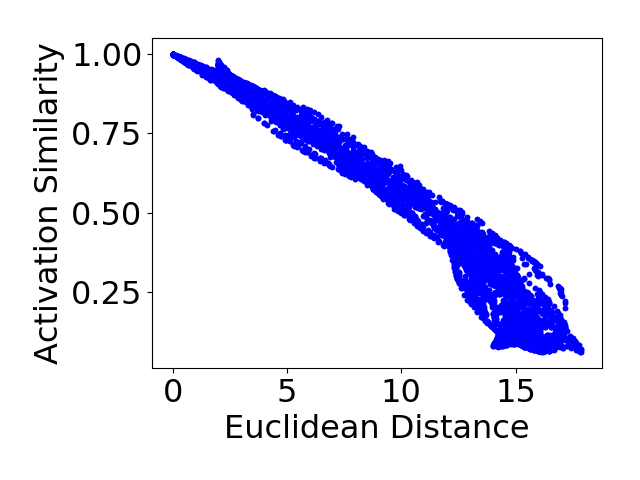
\includegraphics[scale=0.41]{Figures/donut_MLPNet_ripple_optimal_activation_all.png}
			\label{fig:activation}}
        \hspace{0.01in}
        	\subfigure[The local elasticity of two-layer neural nets with sigmoid activation function on the torus function.]{
			\centering
			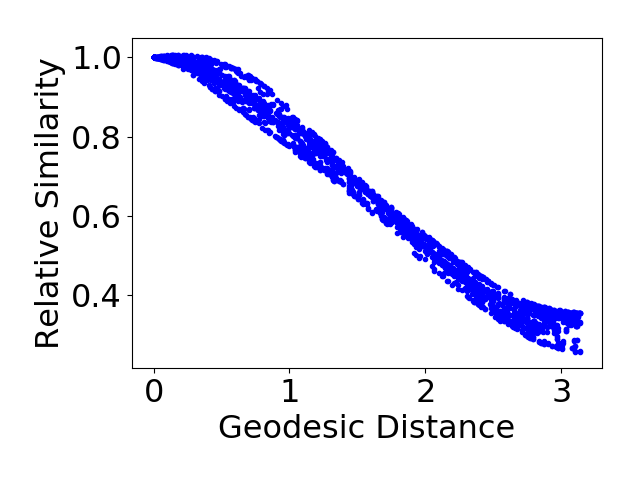
\includegraphics[scale=0.41]{Figures/donut_MLPNetSigmoid_ripple_optimal.png}
			\label{fig:sigmoid}}
        \hspace{0.01in}
        \caption{The activation analysis and the activation function analysis of neural nets local elasticity. The Pearson correlation between the cosine similarity based on activation patterns and the corresponding Euclidean distances is $-0.97$ on the torus function. The cosine similarity within activation patterns indicates the Euclidean distance between two data points. The Pearson correlation between the relative similarity based on  two-layer neural nets with sigmoid activation function and the geodesic distance is $-0.99$. It indicates that two-layer neural nets with sigmoid activation function also have a strong local elastic effect.}
		\label{fig:activation-sigmoid}
\end{figure*}

\paragraph{Architectures.}
%\label{subsec:architectures}
We use $40960$ neurons with ReLU activation function for two-layer neural nets in simulations and experiments. We use $8192$ neurons for each hidden layer with ReLU activation function in three-layer neural networks in simulations. The ResNet we use in experiments is a three-layer net that contains $4096$ neurons and a ReLU activation function in each layer. The CNN for MNIST we use in experiments is the same architecture as that in \url{https://github.com/pytorch/examples/blob/master/mnist/main.py}.


\paragraph{Weights.}
%\label{subsec:random-vs-optimal}
%{\bf Parameter Initialization.} 
As discussed in Section \ref{sec:local-elast-based}, parameter initialization is important for local elasticity based clustering methods. We find that the optimal setting always outperforms the random setting. It supports the intuition that we can learn detailed features of primary examples to better distinguish them from auxiliary examples. 
%More details can be found in Appendix \ref{subsec:random-vs-optimal}. 
The results of two different types of parameter initialization are shown in Table \ref{table:ramdom-vs-optimal}.

\paragraph{Auxiliary examples.}
%\label{subsec:auxiliary-examples}
%{\bf Auxiliary Examples.} 
% Another important aspect of our methods is the choice of auxiliary examples. 
In general, we can choose those samples that are similar to primary examples as auxiliary examples, so they can help neural nets better learn primary examples. We analyze the primary examples pair $5$ and $8$ in MNIST with $6$ different settings of auxiliary examples. We find that the choice of auxiliary examples are crucial. For example, in our case $9$ is close to $5$ and $3$ is close to $8$ based on $K$-means clustering results, so that we can choose $9$ and $3$ as auxiliary examples for models to better distinguish $5$ and $8$. 
%More details can be found in Appendix \ref{subsec:auxiliary-examples}.
%Show an example here and list different auxiliary examples. We use batch size 50 for all experiments, except 5-8-3-3 on BCE loss because it overfits at some points where we cannot get the elastic kernel and elastic similarity results, we simply use the batch size 500 for it.\\
The results of different auxiliary examples for $5$ vs $8$ on MNIST are shown in Table \ref{table:auxiliary-examples}.

\paragraph{Normalized kernelized similarity.}
%%\label{subsec:normalized-kernel}
%{\bf Normalized Kernelized Similarity.}
The normalized kernelized similarity is
\[
\bSk(\bx, \bx'):= \Sk(\bx, \bx')/\sqrt{\Sk(\bx, \bx) \Sk(\bx', \bx')}.
\]
The normalized kernelized similarity can achieve more stable local elasticity. We compare clustering algorithms based on kernelized similarity and normalized kernelized similarity in MNIST. We find that the performance of the normalized kernelized similarity based methods is slightly better than that of kernelized similarity based methods with the $\ell_2$ loss, although this conclusion no longer holds true with cross-entropy loss. 
%More details can be found in Appendix \ref{subsec:normalized-kernel}. 
The results of the normalized kernelized similarity are shown in Table~\ref{table:normalized-kernel}.



\paragraph{Expected relative change.}
%\label{subsec:change}
%{\bf Expected Relative Change Analysis.}
We compute the average relative change of two-layer neural nets and linear neural networks fitting the torus function. The average relative change of two-layer neural nets and linear neural networks are $0.44$ and $0.68$, indicating that SGD updates of two-layer neural nets are more local than that of two-layer linear neural networks. These findings further support our local elasticity theory of neural nets.

\paragraph{Activation patterns.}
%\label{subsec:activation}
%{\bf Activation Analysis.} 
The key difference between our methods and linear baselines is nonlinear activation. We analyze the relations between the patterns of ReLU activation function of two-layer neural nets and corresponding Euclidean distances. For each input $\mbf{x}$, we use $\mbf{a}$ to denote the binary activation pattern of each neuron. The similarity between binary activation patterns is computed from the cosine similarity function. We find that the activation similarity is linearly dependent on the Euclidean distance, meaning that closer points in the Euclidean space will have more similar activation patterns. 
%More details can be found in Appendix \ref{subsec:activation}. 
%The activation analysis for two-layer neural nets on the torus function are shown in Figure \ref{fig:activation}. 
 The activation analysis of neural nets local elasticity are shown in Figure~\ref{fig:activation}.

\paragraph{Activation functions.}
%%\label{subsec:sigmoid}
%{\bf Activation Function Analysis.} 
We experiment on another standard activation function, sigmoid, to see its local elasticity. We find that sigmoid can also provide neural nets with the local elasticity.
%More details can be found in Appendix \ref{subsec:sigmoid}.
%The results are shown in Figure \ref{fig:sigmoid}.
The local elasticity of two-layer neural nets with sigmoid activation function on the torus function is shown in Figure \ref{fig:sigmoid}.

\paragraph{Data normalization.}
%\label{subsec:data-normalization}
The performance of the methods without data normalization are shown in Table \ref{table:data-normalization}. The results show that normalization is important for our methods, which are consistent with our analysis in Section \ref{sec:conclusion}.


%%% Local Variables:
%%% mode: latex
%%% TeX-master: "paper"
%%% End:
